\documentclass{article}
\usepackage{amsmath}
\usepackage{graphicx}
\usepackage{fancyhdr}
\usepackage{array}
\usepackage{booktabs}
\usepackage[sorting=none]{biblatex}
\usepackage[margin=1in]{geometry}
\usepackage{listings}

\lstset{
    language=Python,                    % تنظیم زبان پایتون
    backgroundcolor=\color{white},      % رنگ پس‌زمینه سفید
    basicstyle=\ttfamily\footnotesize,  % استفاده از فونت monospaced
    keywordstyle=\color{blue},           % رنگ کلمات کلیدی
    commentstyle=\color{green},         % رنگ کامنت‌ها
    stringstyle=\color{red},            % رنگ رشته‌ها
    numbers=left,                       % شماره‌گذاری خطوط
    numberstyle=\tiny\color{gray},      % استایل شماره‌های خطوط
    stepnumber=1,                       % شماره‌گذاری هر خط
    numbersep=5pt,                      % فاصله شماره‌گذاری از کد
    showspaces=false,                   % نمایش فضاها
    showstringspaces=false,             % نمایش فضاها در رشته‌ها
    showtabs=false,                     % نمایش تب‌ها
    frame=single,                       % نمایش قاب دور کد
    rulecolor=\color{black},            % رنگ قاب دور کد
    tabsize=2,                          % اندازه تب‌ها
    captionpos=b,                       % عنوان در پایین قرار می‌گیرد
    breaklines=true,                    % تقسیم خط‌های طولانی
    breakatwhitespace=true              % تقسیم در فضای خالی
}
\usepackage[hidelinks]{hyperref}
\usepackage{subfigure}
\hypersetup{
    colorlinks=true,
    linkcolor=teal,
    filecolor=magenta,      
    urlcolor=teal,
    citecolor = teal
    }
\usepackage{xcolor}
\usepackage{xepersian}
\usepackage{fontspec}
\setlength\headheight{28pt} 
\addbibresource{bibliography.bib}
\settextfont[Scale=1.2]{IRLotus.TTF}
\setlatintextfont[Scale=1]{Times New Roman}
\renewcommand{\baselinestretch}{1.5}
\pagestyle{fancy}
\fancyhf{}
\rhead{
\includegraphics[width=1cm]{FaultD.png}امتحان میانترم درس یادگیری ماشین}
\lhead{\thepage}
\lfoot{علیرضا امیری}
\renewcommand{\headrulewidth}{1pt}
\renewcommand{\footrulewidth}{1pt}
\AtBeginDocument{
	\def\chapterautorefname{فصل}%
	\def\sectionautorefname{پاسخ سوال}%
	\def\subsectionautorefname{بخش}%
	\def\subsubsectionautorefname{بخش}%
	\def\equationautorefname{رابطهٔ}%
    \def\lstlistingautorefname{برنامۀ}%
}
\renewcommand{\lstlistingname}{Code}
\begin{document}

\begin{titlepage}
\begin{center}

  \begin{figure}[h!]
 	\centering
 	\subfigure{
 		
\includegraphics[width=0.43\columnwidth]{KNTULogo.pdf}
 		\label{fig:FD3M4sav43i22ngCdW2}
 	}
 	\subfigure
 	{
 		
\includegraphics[width=0.33\columnwidth, height=0.45\columnwidth]{Fault}
 		\label{fig:FD3Msav43i22ngCdW2}
 	}
 \end{figure}
 
 % 
\includegraphics[width=0.5\textwidth]{KNTULogo.pdf}\\
 
\vfill
        
\Huge
\textbf{یادگیری ماشین}\\
\textbf{آزمون میان ترم}\\
        
\vfill
        
\begin{table}[ht]
    \centering
    \huge
    \begin{tabular}{|c|c|}
    \hline
    نام و نام خانوادگی & علیرضا امیری\\
    \hline
    شمارۀ دانشجویی &  40202414\\
    \hline
    تاریخ & خرداد ماه 1404\\
    \hline
    \end{tabular}
\end{table}
\end{center}
\end{titlepage}


\href{https://colab.research.google.com/drive/1nAa6jAqZ1ZJrHdWbSQSdEJEAOdABDY1T?usp=sharing}{لینک کولب فایل}

\tableofcontents

\section{سوال 1، سوالات هماهنگ شده}

\subsection{پاسخ سوال هماهنگ شده اول}
برای کلاس بندی دو دسته داده که هر یک دارای توزیع نرمال گوسی با میانگین $\mu$، کوواریانس $\sigma$ و ویژگی های $x$ هستند، از روابط احتمالی این توزیع ها و تعریف توزیع نرمال به شرح زیر استفاده می کنیم.
\begin{equation}
	p(\mathbf{x}\mid C_i)
	= \mathcal{N}\bigl(\mathbf{x};\boldsymbol\mu_i,\Sigma_i\bigr)
	= \frac{1}{(2\pi)^{d/2}\,\lvert\Sigma_i\rvert^{1/2}}
	\exp\!\Bigl(-\tfrac12(\mathbf{x}-\boldsymbol\mu_i)^\top\Sigma_i^{-1}(\mathbf{x}-\boldsymbol\mu_i)\Bigr),
	\quad i=1,2.
\end{equation}

حال، برای دسته بندی این دو کلاس، طبق رابطه ی زیر با استفاده از لگاریتم likelihood،و با فرض $P(C_1)=P(C_2)$ خواهیم داشت:
\begin{equation}
	  \delta(\mathbf{x})
	=\ln p(\mathbf{x}\mid C_1)\;-\;\ln p(\mathbf{x}\mid C_2)
	\;<>_{C_2}^{C_1}0.
\end{equation} 

با جایگذاری فرم گوسی داده ها در این رابطه، رابطه ی تصمیم گیری به فرم کوادراتیک به صورت زیر به دست می آید:
\begin{equation}
	\begin{aligned}
		\delta(\mathbf{x})
		&=\Bigl[-\tfrac12(\mathbf{x}-\boldsymbol\mu_1)^\top\Sigma_1^{-1}(\mathbf{x}-\boldsymbol\mu_1)
		-\tfrac12\ln|\Sigma_1|\Bigr]\\
		&\quad -\Bigl[-\tfrac12(\mathbf{x}-\boldsymbol\mu_2)^\top\Sigma_2^{-1}(\mathbf{x}-\boldsymbol\mu_2)
		-\tfrac12\ln|\Sigma_2|\Bigr]\\
		&=-\tfrac12(\mathbf{x}-\boldsymbol\mu_1)^\top\Sigma_1^{-1}(\mathbf{x}-\boldsymbol\mu_1)
		+\tfrac12(\mathbf{x}-\boldsymbol\mu_2)^\top\Sigma_2^{-1}(\mathbf{x}-\boldsymbol\mu_2)
		-\tfrac12\ln\frac{|\Sigma_1|}{|\Sigma_2|}.
	\end{aligned}
\end{equation}
\begin{equation}
	\mathbf{x}^\top\bigl(\Sigma_2^{-1}-\Sigma_1^{-1}\bigr)\mathbf{x}
	+2\bigl(\boldsymbol\mu_1^\top\Sigma_1^{-1}-\boldsymbol\mu_2^\top\Sigma_2^{-1}\bigr)\mathbf{x}
	+c
	, 
	c=\boldsymbol\mu_2^\top\Sigma_2^{-1}\boldsymbol\mu_2
	-\boldsymbol\mu_1^\top\Sigma_1^{-1}\boldsymbol\mu_1
	-\ln\frac{|\Sigma_2|}{|\Sigma_1|}.
\end{equation}
که با در نظر داشتن متغیر ویژگی های $x$ و عبارت $\mathbf{x} \mathbf{x}^\top = \mathbf{x}^2
$ فرمت کوادراتیک این معادله مشخص میشود. حال، با تغییر مقادیر میانگین و کوواریانس، می توانیم سطوح مختلفی را به دست بیاوریم. به عنوان مثال، در صورتی که مقادیر کوواریانس دو کلاس با یکدیگر برابر باشد، آنگاه $\Sigma_1=\Sigma_2=\Sigma$ و در نتیجه $\Sigma_2^{-1}-\Sigma_1^{-1}=0$ و در نهایت با حذف ضریب بخش درجه 2 این معادله، صفحه ی تصمیم به فرمت خطی به صورت زیر به دست می آید:
\begin{equation}
	(\boldsymbol\mu_1-\boldsymbol\mu_2)^\top\Sigma^{-1}\,\mathbf{x}
	\;-\;\tfrac12\bigl(\boldsymbol\mu_1^\top\Sigma^{-1}\boldsymbol\mu_1
	-\boldsymbol\mu_2^\top\Sigma^{-1}\boldsymbol\mu_2\bigr)
	=0,
\end{equation}

به عنوان مثال، حالت های مختلف برای تغییرات میانگین و کوواریانس داده های کلاس ها در 
\autoref{fig:1}
رسم شده است.
\begin{figure}[h!]
	\centering
	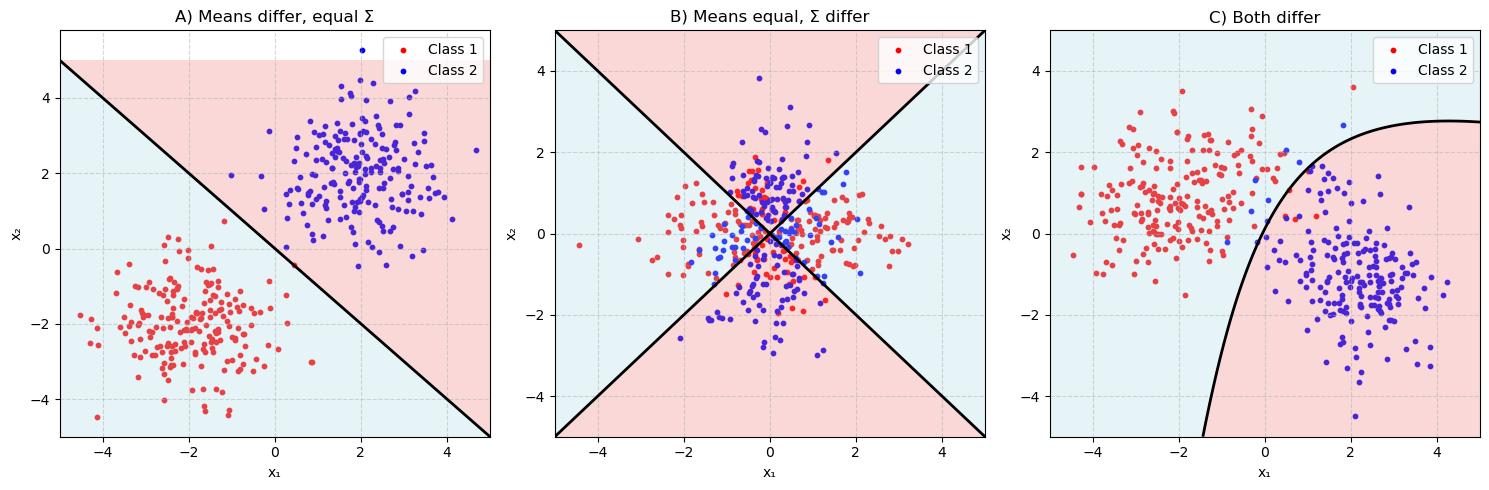
\includegraphics[width=1\linewidth]{1}
	\caption{وضعیت های مختلف صفحه تصمیم با تغییر میانگین و کوواریانس}
	\label{fig:1}
\end{figure}

\clearpage
\subsection{پاسخ سوال هماهنگ شده دوم}
در صورتی که تابع توزیع احتمال را در اختیار داشته باشیم، اولین گام برای تولید نمونه هایی که دارای توزیعی مطابق با این تابع باشند، محاسبه ی تابع توزیع احتمال تجمعی یا به اختصار CDF است. بنابراین، ابتدا با محاسبه ی انتگرال، این تابع را محاسبه می کنیم:
\begin{equation}
	F(x) = \int_{-\infty}^{x} f(t) dt
\end{equation}
آنگاه با استفاده از وارون تابع CDF و وارد کردن داده های تصادفی به آن، داده هایی با توزیع مورد نظر بسازیم. این فرایند به طریق زیر انجام خواهد شد:
\begin{equation}
	x = F^{-1}(u) \Rightarrow x \sim f(x)
\end{equation}
برای راحتی در این بخش، می توان داده های تصادفی را با استفاده از دستور $Uniform(0,1)$ ایجاد کرد. در این حالت، با جایگذاری این داده ها به عنوان ورودی $ F^{-1}(u)$، می توانیم داده های مورد نظر را به دست بیاوریم. با این حال، این روش تنها در حالتی برقرار است که بتوانیم از CDF به دست آمده وارون بگیریم که این در همه ی شرایط برقرار نیست. علاوه بر این، فرایند تولید اعداد با توزیع یکنواخت نیز در اینجا توضیح داده نشده است که در ادامه به آن خواهیم پرداخت.
برای ساخت اعداد تصادفی، الگوریتم های مختلفی مانند $Linear Congruential Generator (LCG)$ و $Mersenne Twister$ تولید می شوند. در این الگوریتم ها، اعداد رندوم در بازه ی 0 تا 1 از تقسیم عددی بزرگ بر $ F^{32}$ یا $ F^{64}$ به دست می آیند. در اینجا، عددی که بر این مقدار تقسیم می شود با استفاده از پارامترهای تصادفی در سخت افزار کامپیوتر ایجاد می شود.

\section{پاسخ سوال 2}
\subsection{الف}
بله، اماطبقه بند بیز در صورتی که تعداد داده ی بی نهایت در اختیار باشد، می تواند طبقه بند بهینه باشد. این در حالی است که شروطی مانند گوسی بودن توزیع داده ها و همچنین متعامد بودن ویژگی ها بر هم برقرار باشد. در این شرایط، به طور ایده آل طبقه بند بیز می تواند در صورت برقراری شرایط بهترین طبقه بند باشد

\subsection{ب}
بله. به دلیل آنکه این توزیع، احتمالات پیشین برای هر پارامتر را دست می آورد که به نوعی رگولاریزیشن محسوب می شود، می تواند وابستگی به پارامتر ها را کم کرده و در نتیجه از اورفیت شدن جلوگیری کند.
\subsection{ج}
بله، به این دلیل که IG به داده هایی که تعداد بیشتری دارند و راحت تر تفکیک می شوند تمایل بیشتری دارد و به آنها در دسته بندی وزن بیشتری می دهد. در حالی که تنوع بیشتر حالت ها لزوما به معنای تفکیک پذیری بیشتر نیست.
\subsection{د}
بله. در صورتی که هیچ خاصیت غیرخطی در توابع فعال ساز استفاده نشود، می توانیم با استفاده از رابطه ی زیر اسثبات کنیم که اعمال یک تابع خطی بر تایع خطی دیگر، به تولید یک تابع خطی منجر می شود.
\begin{equation}
	f(x) = W_2 (W_1 x + b_1) + b_2 = W x + b
\end{equation}

\subsection{ه}

\section{پاسخ سوال 3}
\subsection{الف}
در این درخت، با فرض ورودی داده شده، ابتدا از شاخه ی ایتدایی شروع می کنیم.
\begin{equation}
	A = 1 \Rightarrow D
	D = 1 \Rightarrow \text{Leaf 4}
\end{equation}

حال با استفاده از این ویژگی ها و وزن های داده شده و بایاس، مقدار نهایی را با استفاده از تابع sign برای مجموع مقادیر به دست آمده حساب می کنیم.
\begin{equation}
	\text{Features} = [B, C, E, F] = [1, 0, 0, 1]
\end{equation}
\begin{equation}
	\text{Weights} = [1, 0, -1, 1]
\end{equation}
\begin{equation}
	\text{Bias} = 1
\end{equation}
\begin{equation}
z = 1 \cdot 1 + 0 \cdot 0 + (-1) \cdot 0 + 1 \cdot 1 + 1 = 3
\end{equation}
\begin{equation}
\hat{y} = \text{sign}(z) = \text{sign}(3) = +1

\end{equation}

که در نتیجه، پاسخ یک برای این مدل به دست می آید.
\subsection{ب}
درخت تصمیم علی رغم اینکه از توابع جداساز خطی استفاده می کند، اما در هر گره، یک جداساز جدید تعریف می کند که در نهایت، به تولید یک مدل تکه ای خطی piecewise منجر می شود که یک مدل خطی محسوب نمی شود. با این حال، این مدل در حالت ساده همواره در هر بخش از دسته بند خطی استفاده می کند. 
در مقایسه ی درخت تصمیم و شبکه عصبی کم عمق، می توان گفت که درخت تصمیم gemneralization بهتری نسبت به شبکه کم عمق دارد و همچنین سریع تر آموزش می بیند. با این حال، این مدل نسبت به نویز و خطا در داده ها حساسیت بیشتری دارد و در صورتی که داده ی نویزی به سیستم داده شود، دچار خاطی بیشتری می شود.  و در صورتی که تفسیرپدیری مدل اهمیت داشته باشد، واضح است که درخت تصمیم مفاهیم فیزیکی و قابل تفسیری دارد که شبکه از آن بی بهره است.
علاوه بر این، درخت تصمیم با فرض متعامد بودن ویژگی هاا عمل می کند و تعامل آنها با هم دیگر را در نظر نمی گیرد، در حالی که مدل کم عمق همچنان می تواند این کار را انجام دهد.

\section{پاسخ سوال 4}
\subsection{پیش پردازش و مدل لجستیک رگرسیون}
در بخش ابتدایی با استفاده از دستور $fetch_covtype$ دیتاست را به محیط پایتون لود کرده و آن را در قالب یک دیتافریم ذخیره می کنیم.

با بررسی این دیتاست، مشاهده می کنیم که هیچ مقدار NAN ندارد و نکته ی مهم در این باره آن است که از ستون 10 به بعد، مقدار فیچر ها به صورت Categorical هستند. این موارد در \autoref{fig:2} مشخص شده است.
\begin{figure}[h!]
	\centering
	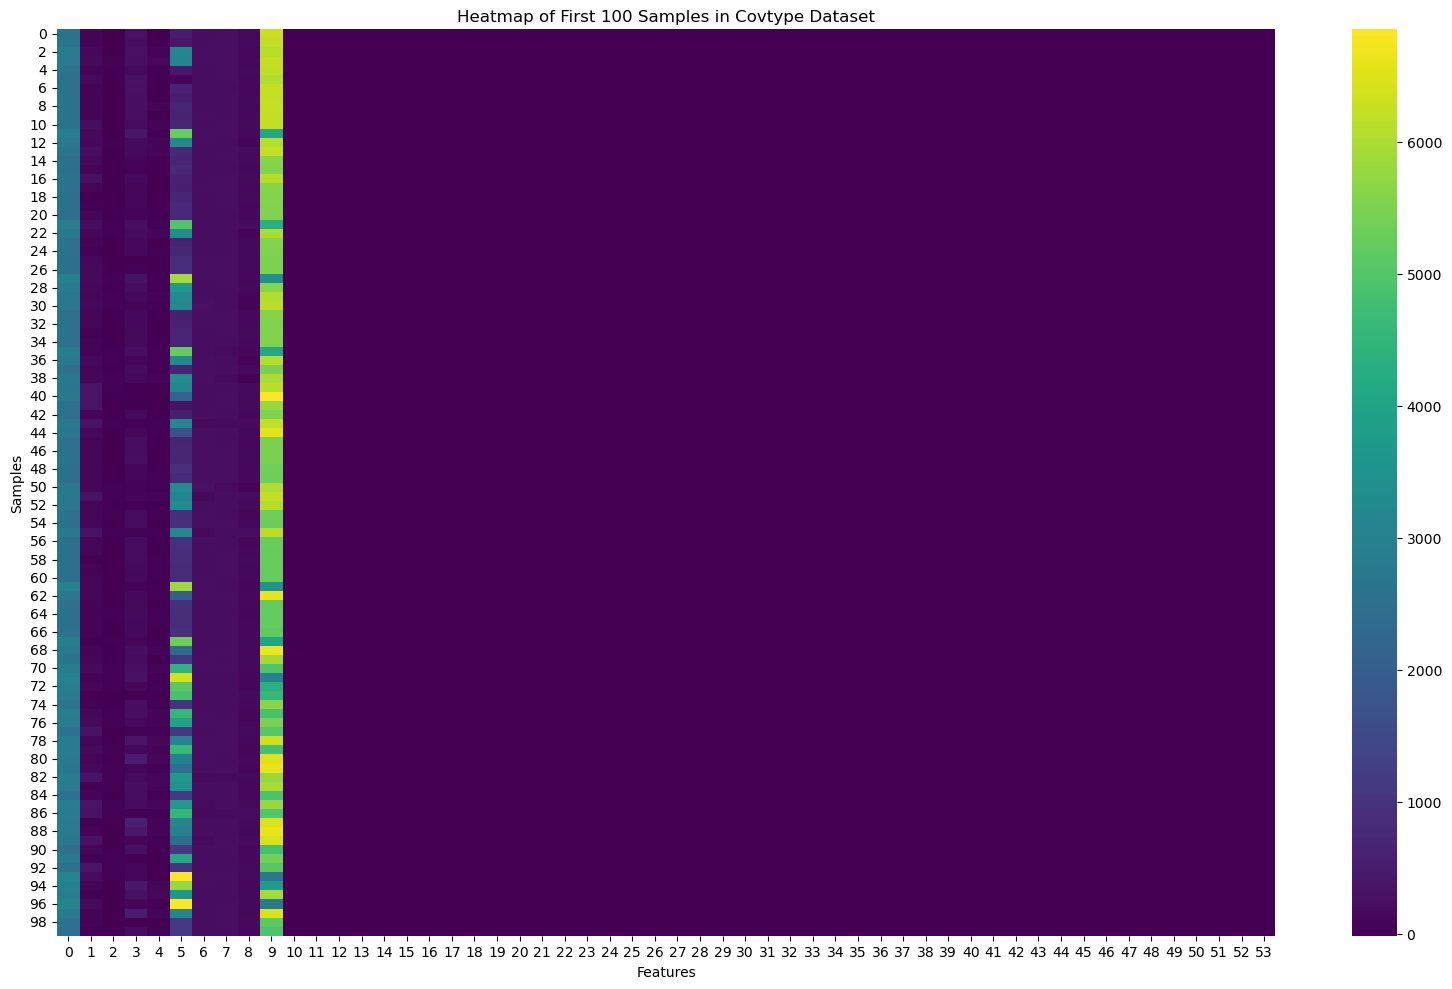
\includegraphics[width=0.7\linewidth]{2}
	\caption[]{نمودار حرارتی دیتاست}
	\label{fig:2}
\end{figure}
\clearpage
بر این اساس، داده های ستون های 10 به بعد را همان طور که هستند نگه داشته و داده های سایر ستون ها را با استفاده از StandardScaler تغییر می دهیم. در نهایت دیتاست به صورت \autoref{fig:3} دست خواهد آمد.
\begin{figure}[h!]
	\centering
	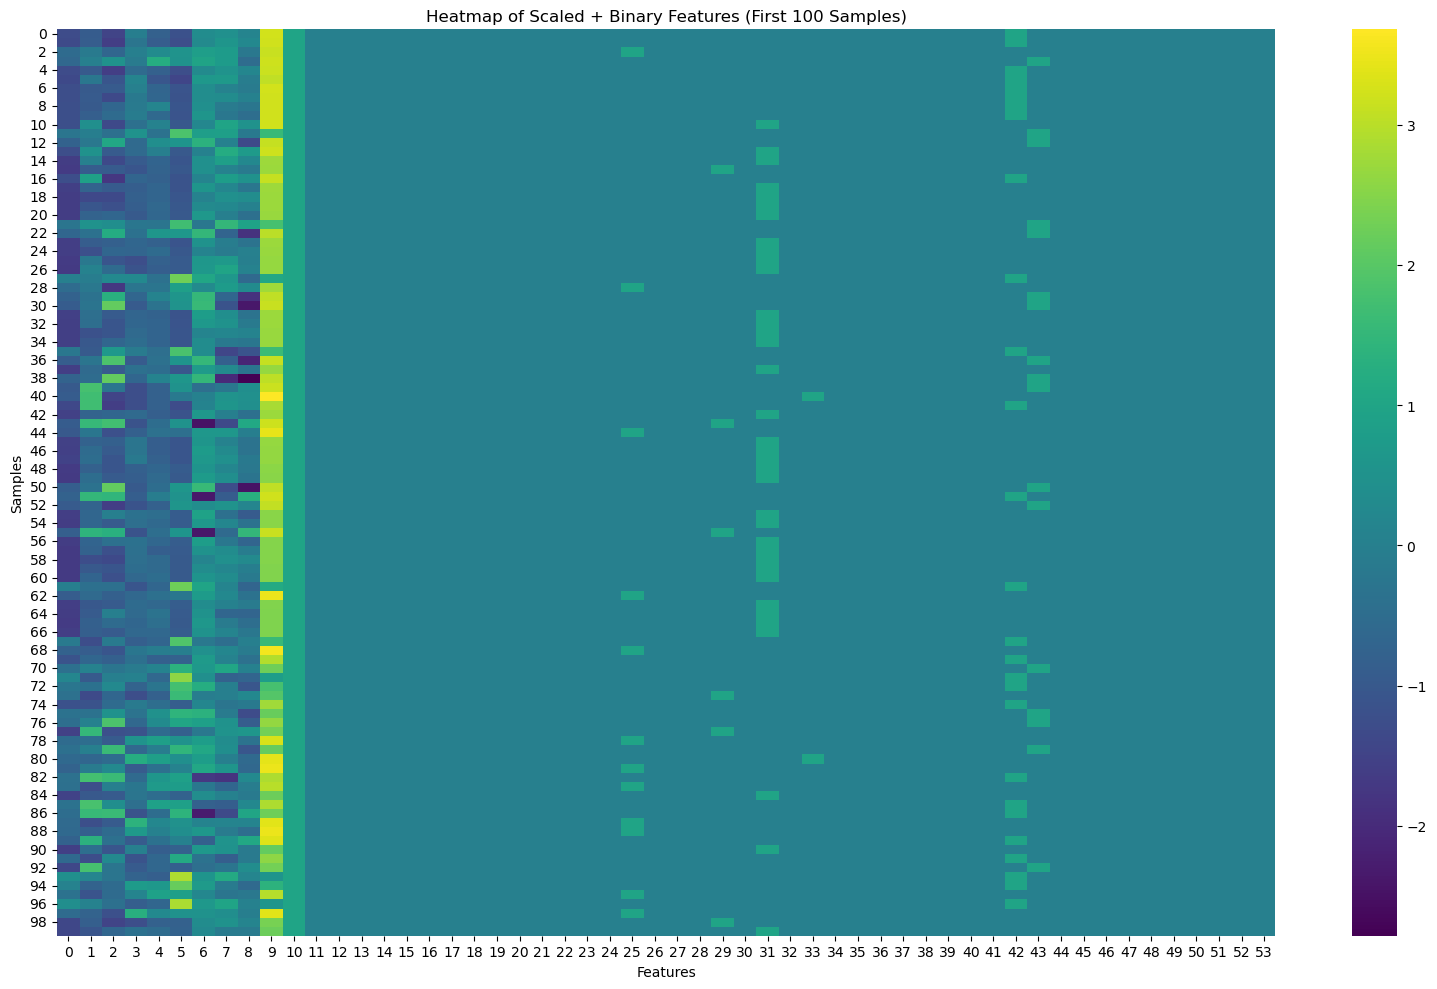
\includegraphics[width=0.7\linewidth]{3}
	\caption[]{نمودار حرارتی دیتاست پس از Scaling}
	\label{fig:3}
\end{figure}
\clearpage
بدون در نظر داشتن این مورد و با آموزش مدل بر دیتاست خام، پاسخ های به دست آمده به صورت زیر بود.
\begin{figure}[h!]
	\centering
	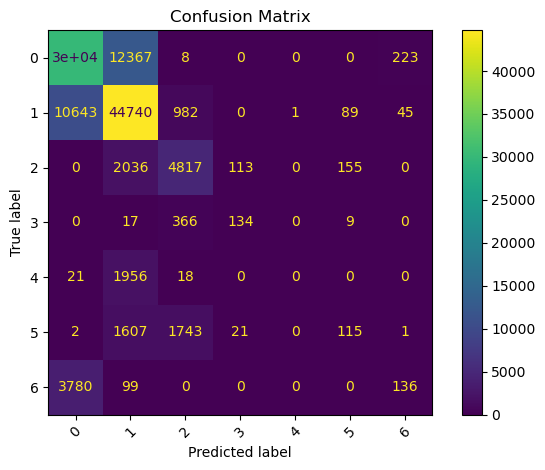
\includegraphics[width=0.7\linewidth]{4}
	\caption[]{نتایج مدل بدون در نظر داشتن ستون های دسته بندی}
	\label{fig:4}
\end{figure}
\clearpage
نتایج به دست آمده از مدل قبل از تغییر ویژگی ها به صورت زیر است:

Accuracy: 0.687598426890872

Precision: 0.65381111874766

Recall: 0.687598426890872

F1 Score: 0.6616133185961008

اما پس از اعمال این تغییرات، نتایج به دست آمده به صورت زیر خواهد بود که می بینیم عملکرد آن بهبود پیدا کرده است. \autoref{fig:5}
\begin{figure}[h!]
	\centering
	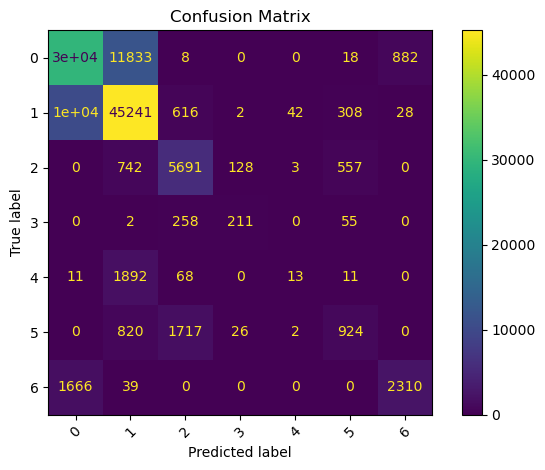
\includegraphics[width=0.7\linewidth]{5}
	\caption{[عملکرد مدل بعد از پردازش ها]}
	\label{fig:5}
\end{figure}
\clearpage
\begin{figure}[h!]
	\centering
	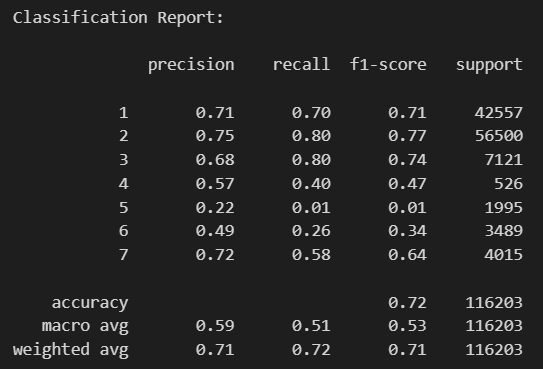
\includegraphics[width=0.7\linewidth]{6}
	\caption[]{classificartion report}
	\label{fig:6}
\end{figure}
\clearpage
در اینجا مشاهده می شود که کلاس های 4 به بعد به دلیل تعداد داده های بسیار کمتر و نامتوازن بودن، عملکرد بدتری دارند نسبت به سایر داده ها. 

\subsection{درخت تصمیم}
در این بهش با آموزش مدل درخت تصمیم بر روی داده های پرئدازش شده در بخش قبل، نتایج بهتری به دست می آوریم.\autoref{fig:7}
\begin{figure}[h!]
	\centering
	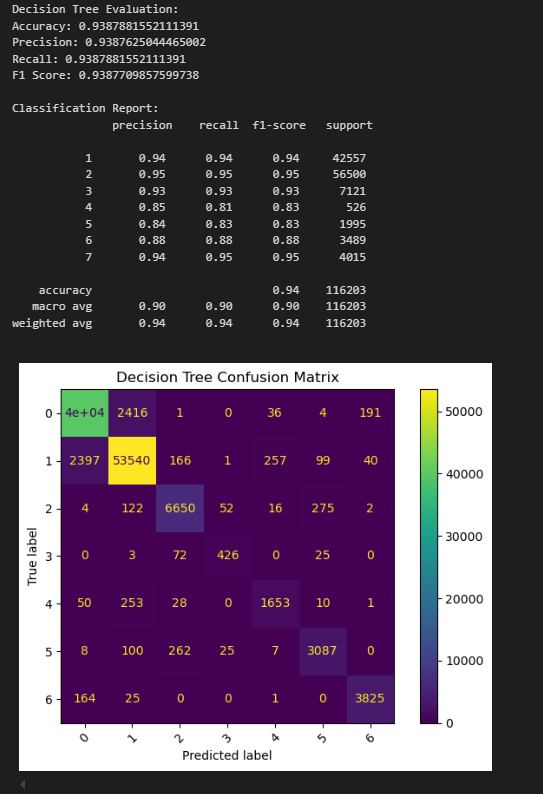
\includegraphics[width=0.7\linewidth]{7}
	\caption[]{نتایج درخت تصمیم}
	\label{fig:7}
\end{figure}
\clearpage
\begin{figure}[h!]
	\centering
	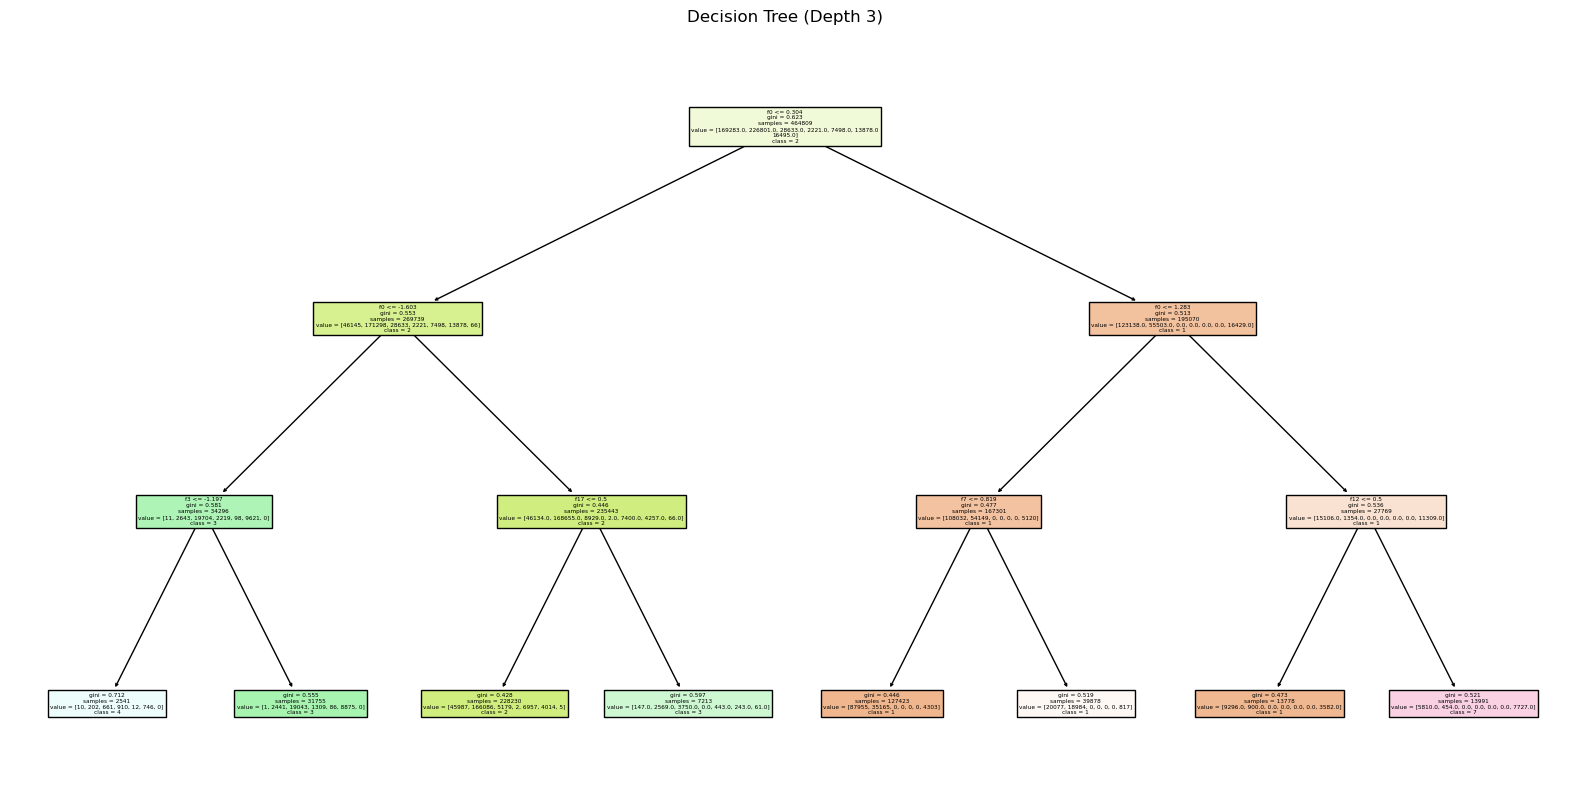
\includegraphics[width=1\linewidth]{8}
	\caption[]{نمودار درخت تصمیم}
	\label{fig:8}
\end{figure}
\clearpage
همچنان مشاهده می کنیم که برای داده هایی که تعداد کمتری داشتند، نتایج با مقدار خطای بیشتری همراه است مانند کلاس های 4 و 5 و 6. اما این عملکرد در مقایسه با لجسنتیک رگرشن پیشرفت بهتری داشته است.
در ادامه ی این بهش، به تنظیم هایپر پارامتر های $max_depth$ و $min_samples_split$ می پردازیم و برای این مقادیر، مدل هایی را آموزش داده و نتایج هر یک را بررسی می کنیم.
\begin{figure}[h!]
	\centering
	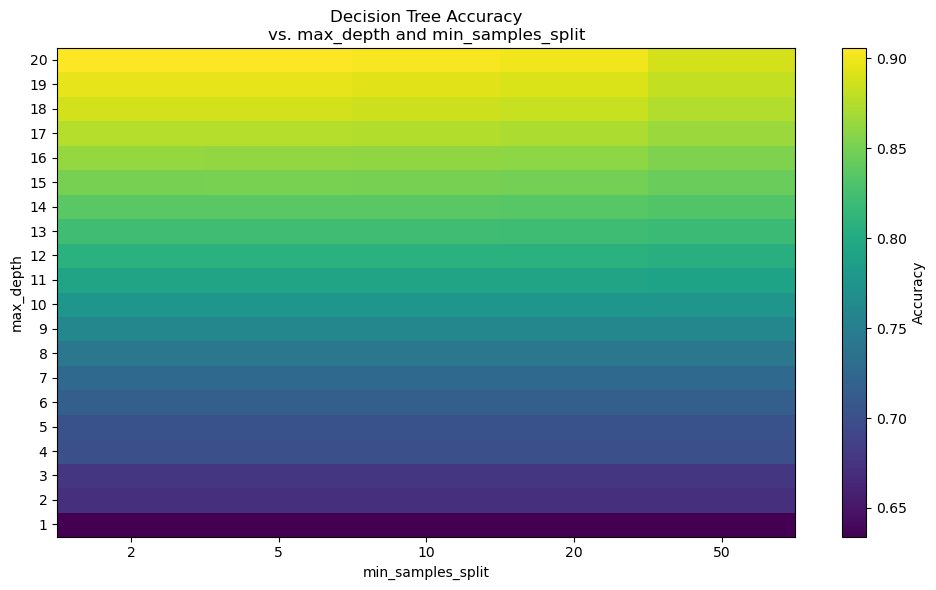
\includegraphics[width=1\linewidth]{16}
	\caption[]{نتایج تغییر پارامتر ها بر عملکرد مدل}
	\label{fig:16}
\end{figure}
چنان که مشاهده می شود، مطابق انتظار با افزایش عمق درخت و کاهش کمتری تعداد نمونه در هر شاخه، دقت سیستم افزایش یافته است. اگرچه در حالت بیشینه، این امر به اورفیت شدن منجر می شود.
با تغییر این پارامتر ها، می توان به ترکیبی دست یافت که هم به داده ها اورفیت نشده باشد و general باشد، و هم دقت کافی را در دسته بتندی داشته باشد.
\clearpage

\section{پاسخ سوال 5}
در این بخش، ابتدا داده ها را دانلود کرده و دیتای آن را بررسی می کنیم. مشاهده می شود که داده ها در سه کلاس دسته بندی شده اند و در مجموع 500 داده قرار دارد که ستون چهارم، لیبل ها هستند.
مشاهده می شود که توزیع داده ها در دو کلاس اول برابر و در کلاس سوم کمتر است .
\begin{figure}[h!]
	\centering
	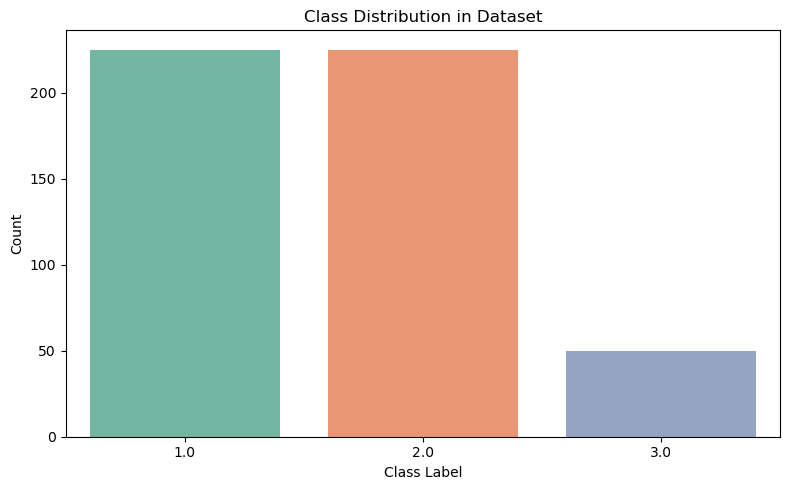
\includegraphics[width=0.7\linewidth]{9}
	\caption[]{توزیع داده ها}
	\label{fig:9}
\end{figure}
\clearpage
بنابراین می توان انتظار داشت که نتیج به دست آمده برای این داده ها در پایان دقت کمتری نیز داشته باشند. در این بخش، ابتدا یک تابع فاصله ی اقلیدوسی به صورت زیر برای سیستم تعریف شد:
\begin{equation}
	d(x_1, x_2) = \sqrt{\sum (x_{1i} - x_{2i})^2}
\end{equation}
با استفاده از این تابع فاصله، الگوریتم KNN مطابق فرایند زیر تعریف شد.

\begin{equation}
	\mathcal{D}_{x_t} = \{(d(x_t, x_i), y_i) \mid x_i \in \text{Train Set}\}
\end{equation}

\begin{equation}
	\mathcal{N}_{k}(x_t) = \text{Top-}k \text{ smallest elements in } \mathcal{D}_{x_t}
\end{equation}

\begin{equation}
	\hat{y}_t = \arg\max_{y} \sum_{(d, y_i) \in \mathcal{N}_k(x_t)} \mathbb{1}_{[y_i = y]}
\end{equation}

\begin{equation}
	\text{Accuracy} = \frac{1}{m} \sum_{i=1}^{m} \mathbb{1}_{[\hat{y}_i = y_i]}
\end{equation}

با آموزش این مدل، نتایج دسته بندی به شرح زیر به دست می آید.\autoref{fig:11}
\begin{figure}[h!]
	\centering
	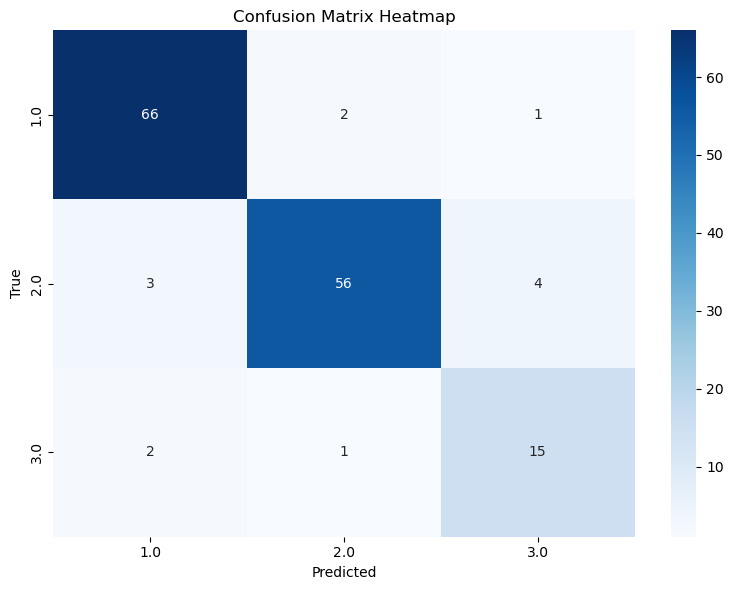
\includegraphics[width=0.7\linewidth]{11}
	\caption[]{نتایج KNN}
	\label{fig:11}
\end{figure}
\clearpage
\begin{figure}[h!]
	\centering
	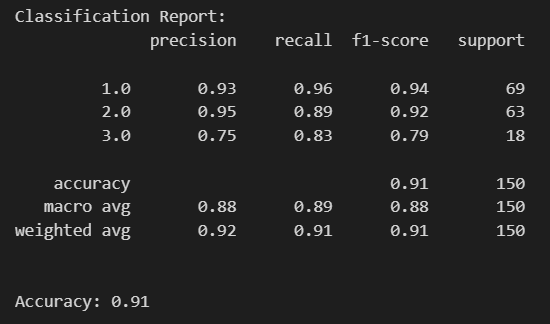
\includegraphics[width=0.7\linewidth]{12}
	\caption{[گزارش دسته بندی KNN]}
	\label{fig:12}
\end{figure}
\clearpage
مشاهده می شود که این مدل توانسته داده ها را به خوبی با دقت 91 درصد دسته بندی کند. برای نمایش توزیع داده های نمونه با استفاده در pca در فضایی کاهش بعد داده شده خواهیم داشت:
\begin{figure}[h!]
	\centering
	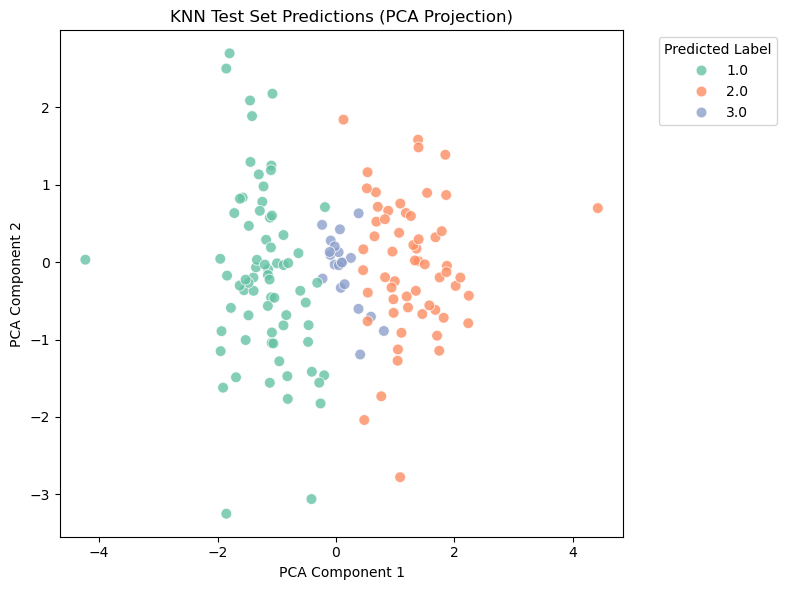
\includegraphics[width=0.7\linewidth]{13}
	\caption{[توزیع با استفاده از pca]}
	\label{fig:13}
\end{figure}
\clearpage
در ادامه، به بررسی تاثیر تغییرات مقدار k در این الگوریتم می پردازیم. این مقادیر از 1 تا 21 تغییر داده شده و دقت مدل برای هر یک در رسم شده است.
\begin{figure}[h!]
	\centering
	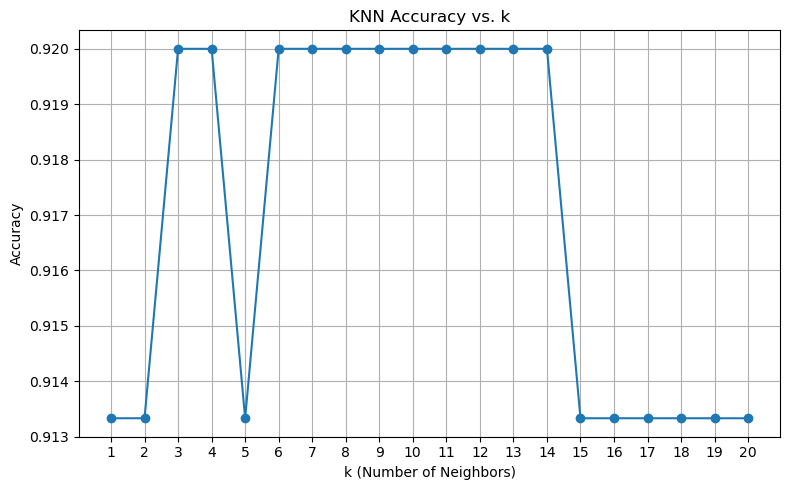
\includegraphics[width=0.7\linewidth]{14}
	\caption{[نمودار تغییرات دقت بر حسب k]}
	\label{fig:14}
\end{figure}
\clearpage
مشاهده می کنیم که تغییرات k تاثیر به سزایی در دقت مدل ندارد در نتیجه استفاده از مقادیر کمتر، برای سادگی الگورتیم توصیه می شود.
در بخش بعدالگوریتم KNN وزن دار تعریف و استفاده شده است.
\begin{figure}[h!]
	\centering
	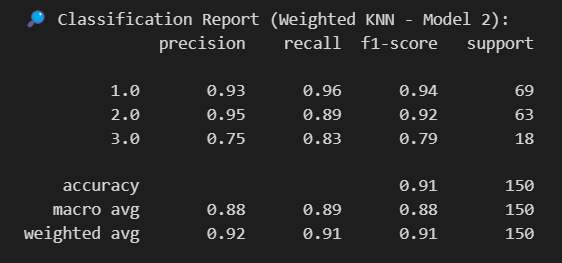
\includegraphics[width=0.7\linewidth]{15}
	\caption{[نتیجه KNN وزن دار]}
	\label{fig:15}
\end{figure}
\clearpage
و مشاهده می شود که تعداد پ
یش بینی شده دقیقا برابر با الگوریتم KNN ساده است و اعمال وزن تاثیری در آن نداشته.
در بخش انتهایی با استفاده از روش cross validation به شرح زیر، عملکرد مدل ه را بررسی می کنیم.
برای هر تایش (fold):
\begin{itemize}
	\item مدل روی $K - 1$ بخش آموزش می‌بیند.
	\item روی بخش باقی‌مانده ارزیابی می‌شود.
	\item دقت برای هر بار تایش به صورت زیر محاسبه می‌شود:
	\[
	\text{Accuracy}_i = \frac{1}{m} \sum_{j=1}^{m} \mathbb{1}[\hat{y}_j = y_j]
	\]
\end{itemize}

این فرآیند برای دو مدل انجام می‌شود:
\begin{itemize}
	\item مدل ۱: KNN معمولی (با رأی‌گیری اکثریت)
	\item مدل ۲: KNN وزنی (با وزن‌دهی معکوس فاصله):
	\[
	w_i = \frac{1}{d(x, x_i) + \epsilon}
	\]
\end{itemize}

در نهایت، دقت میانگین محاسبه می‌شود:
\[
\text{Mean Accuracy} = \frac{1}{K} \sum_{i=1}^{K} \text{Accuracy}_i
\]


آنگاه نتایج این cross validation به صورت زیر به دست می آید که می بینیم مدل دوم اندکی بهتر از مدل اول عمل کرده است.
\begin{figure}[h!]
	\centering
	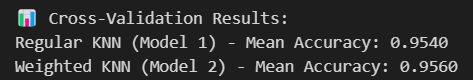
\includegraphics[width=0.7\linewidth]{17}
	\caption[]{cross validation}
	\label{fig:17}
\end{figure}
\clearpage
\end{document}

